\documentclass[aspectratio=169]{beamer}

\usepackage[utf8]{inputenc}
\usepackage[T1]{fontenc}
\usepackage[brazil]{babel}
\usepackage{amsmath,amssymb}
\usepackage{tikz,xcolor,graphicx}
%tikz stuff
\usetikzlibrary{calc}
\usetikzlibrary{positioning}


\input{C_macros}

%\usetheme{Madrid}
%\usecolortheme{seahorse}

% --- Macros usadas no texto original (ajuste se já tiver um pacote próprio) ---
%\newcommand{\R}{\mathbb{R}}
%\newcommand{\E}{\mathbb{E}\,}
%\newcommand{\eE}[1]{\mathbb{E}\!\left[#1\right]}
%\newcommand{\ProbE}[1]{\mathbb{P}\!\left(#1\right)}
%\newcommand{\Ind}[1]{\mathbb{1}_{#1}}
%\newcommand{\colch}[1]{\{#1\}}
%\newcommand{\conj}[1]{\{#1\}}
%\newcommand{\tq}{:\,}
%\newcommand{\teto}[1]{\lceil #1 \rceil}

\title{Dominância estocástica e acoplamento}
\subtitle{Para análise do QS}

\author{J.D.} \date{\today}

\begin{document}

\begin{frame}
  \titlepage
\end{frame}

\begin{frame}{Roteiro}
  \tableofcontents
\end{frame}

\section{A distribuição uniforme contínua}
% --------------------------------------------------------------------
\begin{frame}{Distribuição uniforme em $[a,b]$}

  \vfill
  
  \phantom{Sejam $a<b$. }$X\sim \mathrm{U}(a,b)$ se $X$ é absolutamente contínua
  
  \vfill
  
  \[
  \text{com densidade} \quad  f(x)=\frac{1}{b-a}\,\Ind{[a,b]}(x)
  \]
  
  \vfill
  
  \[
   \text{com distrib.~acumulada} \quad \boxed{F_X(t) \coloneqq \ProbE{X\leq t}} = \begin{cases}
      0, & t<a,\\[2pt]
      \dfrac{t-a}{b-a}, & a\leq t\leq b,\\[6pt]
      1, & t>b.
    \end{cases}
  \]
  \vfill
  
\end{frame}
% --------------------------------------------------------------------
\begin{frame}{Distribuição uniforme em $[0,1]$}
  \vfill
  
  \phantom{Sejam $a<b$. }$X\sim \mathrm{U}(0,1)$ se $X$ é absolutamente
  contínua
  \vfill
  
  \[
  \text{com densidade} \quad   f(x)= 1\cdot \Ind{[0,1]}(x)
  \]
 
  \vfill
  
  \[
   \text{com distrib.~acumulada} \quad  F_X(t)=\begin{cases}
      0, & t<0,\\[2pt]
      t, & 0\leq t\leq 1,\\[6pt]
      1, & t>1.
    \end{cases}
  \]
\vfill
  
  \end{frame}
% --------------------------------------------------------------------
\section{Transformação  da probabilidade}

\begin{frame}{Transformação integral da probabilidade} 
  \begin{block}{Proposição}
    Seja $F$ uma função de distribuição acumulada qualquer e defina
    \[
      F^{-1}(u)\coloneqq \inf\{x\in\R : F(x)\geq u\}, \qquad \forall u\in(0,1).
    \]
    Se $U\sim \mathrm{U}(0,1)$, então $F^{-1}(U)$ tem função de
    distribuição $F$.
  \end{block}

  \vfill
  
  \begin{itemize}
    \item Vale para \textbf{qualquer} $F$ --- discreta, contínua, mista.
    \item $F^{-1}$ é a \emph{inversa generalizada}: coincide com a
          inversa usual quando $F$ é bijetora.
        \item Demonstração (omitida) usa monotonicidade e continuidade à
          direita de $F$.
  \end{itemize}
\end{frame}
% --------------------------------------------------------------------
\begin{frame}{Por que isso importa}
  \begin{center}
    \Large
    {\textbf\textit{{Qualquer}}} distribuição pode ser \textbf{simulada} a partir de uma
    única variável uniforme.
  \end{center}
  \vfill
  \begin{itemize}
    \item Base de todos os algoritmos probabilísticos que geram v.a.'s
          a partir de \texttt{random()}.
    \item Mais adiante: usar o \textbf{mesmo} $U$ para gerar duas
          variáveis diferentes cria uma \textbf{dependência
          controlada} entre elas --- a ideia central de
          \emph{acoplamento}.
  \end{itemize}
\end{frame}
% --------------------------------------------------------------------
\begin{frame}{Simulação de uma Bernoulli}
  \begin{columns}[T]
    
  \begin{column}{0.48\textwidth}
    $X\sim \mathrm{Bernoulli}(p)$
    \[
      F_X(t) = \begin{cases}
        0, & t < 0 \\
        1-p, & 0 \leq t < 1 \\
        1, & t \geq 1.
      \end{cases}
    \]
  \end{column}
  
  \begin{column}{0.48\textwidth}
    \begin{center}
      \begin{tikzpicture}[scale=1.3]
        % Eixos
        \draw[->] (-1.5,0) -- (2.5,0) node[right] {$t$};
        \draw[->] (0,-0.3) -- (0,1.5) node[above] {$F_X(t)$};
      
      % Marcação no eixo y
      \draw (0,1) -- (-0.05,1) node[left] {$1$};
      \draw[dashed, lightgray] (0,1) -- (1,1);

      \draw (0,.53) -- (-0.05,.53) node[left] {$1-p$};
%      \draw[dashed, lightgray] (0,.3) -- (1,.3);
      
      % Marcação no eixo x
      \draw (0,0.05) -- (0,-0.05) node[below] {$0$};
      \draw (1,0.05) -- (1,-0.05) node[below] {$1$};
      
      % Trecho para t <= 0 : F(t) = 0
      \draw[thick] (-1.5,0) -- (0,0);
      \draw[fill=white] (0,0) circle (0.05); % bola aberta

      % Trecho para 0< t < 1 
      \draw[thick] (0,.53) -- (1,.53);
      \draw[fill=black] (0,0.53) circle (0.05); % bola aberta
      \draw[fill=white] (1,0.53) circle (0.05); % bola aberta
      
      % Trecho para t >= c: F(t) = 1
      \draw[thick] (1,1) -- (2.5,1);
      \draw[fill=black] (1,1) circle (0.05); % bola fechada
    \end{tikzpicture}
  \end{center}
  \end{column}

\end{columns} \pause

\[
    F_X^{-1}(u) = \inf \conj{ x \tq F_X(x) \geq u } =
    \begin{cases}
      0, & u \leq 1-p \\
      1, & u > 1-p
    \end{cases}
  \]

  \pause

  
  \[
    U \sim \mathrm{U}(0,1) \Longrightarrow X' = F_X^{-1}(U) =
    \Ind{\colch{U > 1-p}} \stackrel{d}{=} X \sim \mathrm{Bernoulli}(p)\]


\end{frame}
% --------------------------------------------------------------------
\begin{frame}{Simulação de uma Bernoulli}

  \begin{center}
    $1-U\sim \mathrm{U}(0,1)$ e $\ProbE{U\leq p}=p$    
  \end{center}
  $$\To$$
  \[ X'\coloneqq \Ind{\colch{U <  p}}  = \Ind{\colch{1-U > 1-p}} \sim \mathrm{Bernoulli}(p)\]

  \bigskip
  
  Por isso, costuma-se escrever de forma simétrica que $U$ nos dá
  \(
  \boxed{X'=  \Ind{\colch{U \leq   p}}}
  \)
\end{frame}
% --------------------------------------------------------------------

\begin{frame}{Simulando um dado justo}
  $Y\in\{1,\dots,6\}$ uniforme discreta:
  \begin{columns}[T]
    
    \begin{column}{0.48\textwidth}
      \[
        F_Y(t) = \sum_{k=1}^{6} \frac{1}{6}\,\Ind{\{k\leq t\}}= 
        \begin{cases}
          0, & t < 1 \\
          1/6, & 1 \leq t < 2 \\
          2/6, & 2 \leq t < 3 \\
          3/6, & 3 \leq t < 4 \\
          4/6, & 4 \leq t < 5 \\
          5/6, & 5 \leq t < 6 \\
          1, & t \geq 6
        \end{cases},
      \]
      constante por partes, com saltos de $1/6$ em cada inteiro.
    \end{column}
    \def\yscale{3}
    \def\xscale{.8}
    \begin{column}{0.48\textwidth}
      \begin{center}
        \begin{tikzpicture}[scale=.85]
          % Eixos
          \draw[->] (-0.5,0) -- (\xscale*7,0) node[right] {$t$};
          \draw[->] (0,-0.3) -- (0,{\yscale*1.15}) node[above] {$F_Y(t)$};
          
          % Marcações no eixo y (múltiplos de 1/6)
          \foreach \k in {1,...,6} {
            \draw (0,{\yscale*\k/6}) -- (-0.08,{\yscale*\k/6})
            node[left] {\scriptsize $\frac{\k}{6}$};
            \draw[dashed,  lightgray, very thin] (-0.5,{\yscale*\k/6}) -- (\k,{\yscale*\k/6});
          }
          
          % Marcações no eixo x
          \foreach \k in {0,...,6} {
            \draw (\xscale*\k,0.1) -- (\xscale*\k,-0.1) node[below] {$\k$};
          }
          
          % Trecho inicial: F(t) = 0 para t < 1
          \draw[thick] (-\xscale*0.5,0) -- (\xscale*1,0);
          \node[circle, draw, fill=white, inner sep=1.3pt] at (\xscale*1,0) {};
          
          % Degraus intermediários
          \foreach \k in {1,...,5} {
            \pgfmathtruncatemacro{\kk}{\k+1}
            \draw[thick] ({\xscale*\k},{\yscale*\k/6}) -- ({\xscale*\kk},{\yscale*\k/6});
            \node[circle, draw, fill=black, inner sep=1.3pt] at ({\xscale*\k},{\yscale*\k/6}) {};
            \node[circle, draw, fill=white, inner sep=1.3pt] at ({\xscale*\kk},{\yscale*\k/6}) {};
          }
          
          % Trecho final: F(t) = 1 para t >= 6
          \draw[thick] ({\xscale*6},\yscale) -- ({\xscale*7},\yscale);
          \node[circle, draw, fill=black, inner sep=1.3pt] at (\xscale*6,\yscale) {};
        \end{tikzpicture}
      \end{center}
    \end{column}
  \end{columns}
\end{frame}
% --------------------------------------------------------------------
\begin{frame}{Simulando um dado justo}

 
  \[
    F_Y^{-1}(u) = k \quad\text{sempre que}\quad \frac{k-1}{6} < u \leq \frac{k}{6}.
  \]

  \[
    \boxed{Y' = F_Y^{-1}(U) = \lceil 6U \rceil}
  \]
  Pela proposição, $Y'$ tem distribuição de um dado justo.
\end{frame}
% --------------------------------------------------------------------

\section{Dominância estocástica e acoplamento}

\begin{frame}{Dominância estocástica e acoplamento}
  \begin{itemize}[<+->]\itemsep=.6cm
  \item \textbf{o mesmo} $U\sim\mathrm{U}(0,1)$ pode gerar várias
    variáveis aleatórias diferentes, cada uma com a distribuição
    correta. Ex.:
    \begin{center}
      $X' \coloneqq \Ind{\colch{U\leq p}} \sim \mathrm{Bernoulli}(p)$ e
      $Y' \coloneqq \lceil 6U \rceil \sim
      \mathrm{Uniforme}(\conj{1,\dots,6})$.
    \end{center}

       
  \item Se eu uso o mesmo $U$ para gerar $X'$ e $Y'$, existe alguma
    relação \emph{pontual} entre $X'$ e $Y'$?

  \item Essa construção — variáveis com as distribuições certas,
    definidas no mesmo espaço, relacionadas pontualmente — é o que
    chamaremos de \textbf{acoplamento}.

  \item Ela vai caracterizar a \textbf{dominância estocástica} entre
    duas distribuições.
  \end{itemize}
\end{frame}


% --------------------------------------------------------------------

\begin{frame}
  \frametitle

  \begin{block}{Dominação estocástica}
    Sejam $X$ e $Y$ variáveis aleatórias reais (não necessariamente
    definidas no mesmo espaço de probabilidade).

    Dizemos que $X$ \emph{domina estocasticamente} $Y$, e escrevemos
    $X \succeq Y$, se
    \[
      \ProbE{ X >  t} \geq
      \ProbE{ Y >  t} 
    \]
    para todo  \(t\in\R\).
  \end{block}

  \vfill\pause

  \begin{columns}[T]
    \begin{column}{0.55\textwidth}
      
      Equivalentemente,

      \begin{equation*}
        F_X(t) \leq F_Y(t)  \quad (\forall t\in\R).
      \end{equation*}
    \end{column}
    \begin{column}{0.38\textwidth}
      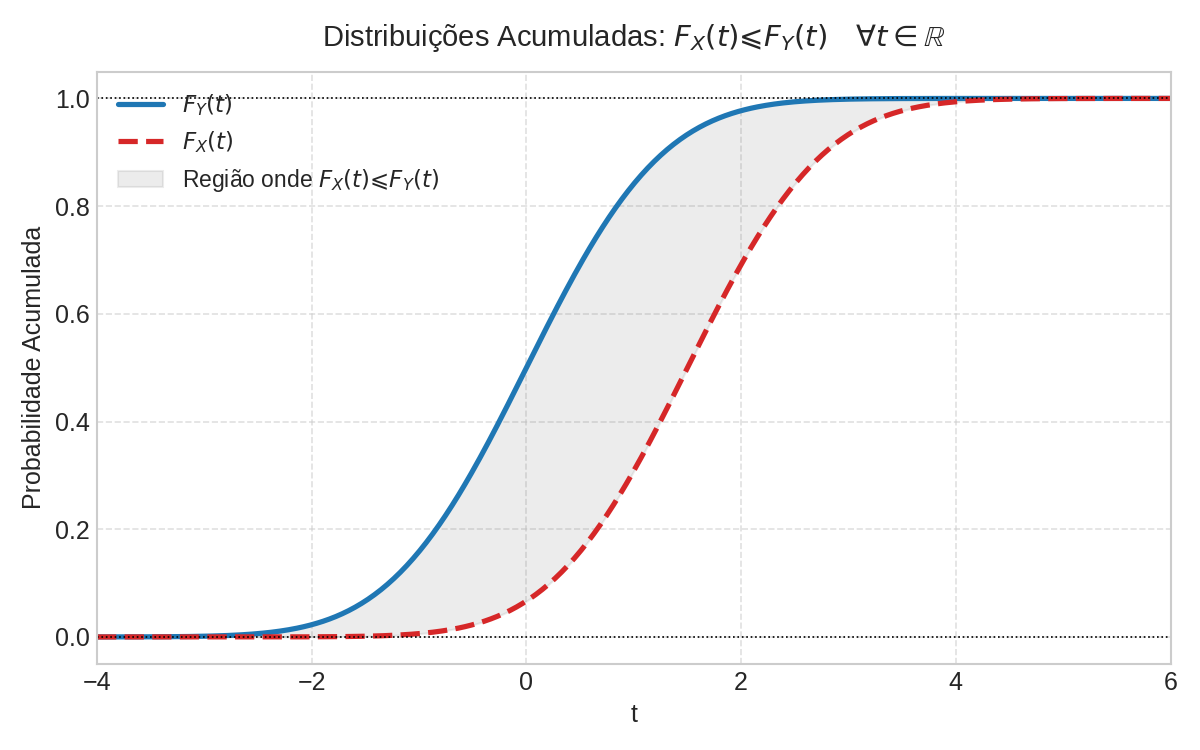
\includegraphics[scale=.13]{domina.png}
    \end{column}
  \end{columns}
  
  \vfill
  
\end{frame}
% --------------------------------------------------------------------
\begin{frame}{$p\geq q \To \mathrm{Bernoulli}(p) \succeq \mathrm{Bernoulli}(q)$} 

  \vfill
  
  $X\sim\mathrm{Bernoulli}(p)$, $Y\sim\mathrm{Bernoulli}(q)$ com
  $p\geq q$.
  
  \vfill
  
  $t < 0$ $\To$ \( \ProbE{ X > t} = \ProbE{ Y > t} =1 \)
  
  \vfill
  
  $0 \leq t < 1$ $\To$ $\ProbE{X > t} = p \geq q = \ProbE{ Y > t }$;

  \vfill
  
  para $t\geq 1$  $\To$ \( \ProbE{ X > t} = \ProbE{ Y > t} = 0 \)

  \vfill

  Logo $X \succeq Y$.

  \vfill
\end{frame}
% --------------------------------------------------------------------
% --------------------------------------------------------------------
\begin{frame}{Acoplamento}


  \vfill
  
   $X\sim\mathrm{Bernoulli}(p)$,
  $Y\sim\mathrm{Bernoulli}(q)$ com $p\geq q$ \quad e \quad $U\sim\mathrm{U}(0,1)$.
  
  \vfill
  
  \[
    X' \coloneqq  \Ind{\colch{U\leq p}} \stackrel d= X,
    \qquad
    Y' \coloneqq  \Ind{\colch{U\leq q}} \stackrel d= Y.
  \]

  \vfill

  \begin{center}
    $\colch{U\leq q} \subseteq \colch{U\leq p}$ $\To$ $(X',Y')$ nunca
  assume o valor $(0,1)$.
  \end{center}

  \vfill
  
  \begin{center}
    $Y'\leq X'$, logo $X\succeq Y$ pois $X'\overset{d}{=}X$,
    $Y'\overset{d}{=}Y$
  \end{center}

   \vfill

   \textbf{Obs} $X,Y$ independentes, então
   $\ProbE{(Y,X)=(1,0)} = q(1-p) >0$ ($q>0$, $p<1$)
  

\end{frame}
% --------------------------------------------------------------------
\begin{frame}
  \frametitle{Acoplamento}

  \vfill
  
  $X$ e $Y$ v.a. (possivelmente definidas em espaços de probabilidade
  diferentes).
  
  \vfill
  
  Um \textbf{acoplamento} de $X$ e $Y$ é um par $(X',Y')$ de variáveis
  aleatórias definidas no mesmo espaço de probabilidade tal que
  
  $$X'\overset{d}{=}X \quad\text{e}\quad Y'\overset{d}{=}Y,$$
  
  \vfill
  
  A distribuição conjunta de $(X',Y')$ é livre: é justamente isso que
  se escolhe de modo conveniente.

\end{frame}
% --------------------------------------------------------------------
\begin{frame}
  \frametitle{Interregno cultural}


  Escolha $(X, Y)$ uniformemente no disco unitário $x^2 + y^2 \leq 1.$

  \vfill
  
  Cada coordenada, vista sozinha, assume qualquer valor em $[-1,1]$.

  \vfill

  Mas, se $X = 0{,}9$, então
  $Y = \pm (1 - 0,81)^{1/2} \approx \pm 0,44$, logo são dependentes.

  \vfill
  
  
  
\end{frame}
% --------------------------------------------------------------------
\begin{frame}

  \vfill
  \begin{block}{{Teorema} de Strassen para ordem estocástica por quantis}
    Para variáveis aleatórias reais $X$ e $Y$, vale $X\succeq Y$ se, e
    somente se, existem variáveis aleatórias $X'\stackrel{d}{=} X$ e
    $Y'\stackrel{d}{=}Y$ definidas num mesmo espaço de probabilidade
    tais que $Y'\leq X'$ com probabilidade~$1$.
  \end{block}
  \vfill
  \begin{block}{Corolário}
    Se $X\succeq Y$, então $\E{Y}\leq\E{X}$ (quando as esperanças
    existem) e, mais geralmente, $\E{f(Y)}\leq\E{f(X)}$ para toda
    função $f$ não decrescente. 
  \end{block}
  \vfill
  
\end{frame}
% --------------------------------------------------------------------
\begin{frame}{$p\geq q \To \mathrm{Binomial}(m,p) \succeq \mathrm{Binomial}(m,q)$}

    Se $X\sim\mathrm{Binomial}(m,p)$ e $Y\sim\mathrm{Binomial}(m,q)$
    com $1\geq p\geq q\geq 0$, então $X\succeq Y$.


  \vfill

  \textbf{Ideia:} somar acoplamentos Bernoulli, um para cada tentativa,
  com o \emph{mesmo} $U_i$ em cada par.

  \vfill

  \begin{itemize}
  \item Já sabemos: $\mathrm{Bernoulli}(p)\succeq\mathrm{Bernoulli}(q)$
    pelo acoplamento $\Ind{\colch{U\leq p}}\geq\Ind{\colch{U\leq q}}$.
  \item Falta: passar de uma tentativa para $m$ tentativas
    independentes.
  \end{itemize}

\end{frame}
% --------------------------------------------------------------------
\begin{frame}

  Sejam $U_1,\dots,U_m$ independentes, $U_i\sim\mathrm{U}(0,1)$, e
  \[
    B_i\coloneqq\Ind{\colch{U_i\leq p}},
    \qquad
    C_i\coloneqq\Ind{\colch{U_i\leq q}},
    \qquad i=1,\dots,m.
  \]

  \vfill

  \begin{enumerate}\itemsep=.2cm
  \item $B_1,\dots,B_m$ são independentes, $\mathrm{Bernoulli}(p)$;\\
    $C_1,\dots,C_m$ são independentes, $\mathrm{Bernoulli}(q)$.
  \item Logo
    \[
      X'\coloneqq\sum_{i=1}^mB_i\sim\mathrm{Binomial}(m,p),
      \qquad
      Y'\coloneqq\sum_{i=1}^mC_i\sim\mathrm{Binomial}(m,q),
    \]
    isto é, $X'\stackrel d=X$ e $Y'\stackrel d=Y$: é um acoplamento.
  \item Como $q\leq p$, $\colch{U_i\leq q}\subseteq\colch{U_i\leq p}$,
    logo $C_i\leq B_i$ para todo $i$ e todo $\omega$. Somando,
    $Y'\leq X'$.
  \end{enumerate}

  \vfill

  Pelo teorema, $X\succeq Y$. \qed

%  \vfill


  %\small
%  $B_i$ e $C_i$ \emph{não} são independentes (mesmo $U_i$), e isso não
%  importa: o acoplamento só exige as distribuições marginais corretas.

\end{frame}
% --------------------------------------------------------------------
\begin{frame}{Ponte com o QS}

  \begin{itemize}\itemsep=.4cm
  \item Aqui $p$ e $q$ são \textbf{constantes}.
  \item No QS, a probabilidade de sucesso é $p_i\geq\alpha$, mas
    $p_i$ \textbf{depende do histórico}:
    \begin{itemize}\itemsep=.2cm
    \item $Z_i=\Ind{\colch{U_i\leq p_i}}$ com $p_i$ aleatório, então
      $\sum_iZ_i$ \emph{não} é binomial;
    \item $Y_i=\Ind{\colch{U_i\leq\alpha}}$ continua i.i.d.\
      $\mathrm{Bernoulli}(\alpha)$;
    \item $Y_i\leq Z_i$ vale com probabilidade $1$.
    \end{itemize}
  \item Mesmo $U_i$, mesma comparação: só muda que a cota inferior
    $\alpha$ substitui o $q$ fixo, e o resultado é uma \emph{dominação}
     $\sum_iZ_i \succeq \sum_i Y_i \sim \mathrm{Binomial}(m,\alpha)$.
  \end{itemize}

\end{frame}
% --------------------------------------------------------------------
% --------------------------------------------------------------------
\section{No \textit{quicksort}}

\begin{frame}{No \textit{quicksort}}

  \begin{itemize}[<+->]\itemsep=.25cm
  \item $S=(x_1,x_2,\dots,x_n)$

  \item $X_{i}= $ número de comparações $x_i:\text{pivô}$

  \item $x_i$ participa de no máximo $\ell$ particionamentos com
    sucesso.

  \item Quando $x_i$ deixa de participar, continua com particionamentos
    \textit{fictícios}, com probabilidade $0{,}76$
    \textit{independentemente} do passado.

  \item $M_i$ o número de particionamentos reais de que $x_i$ participa

   \item $\tau_i$ o instante do $(\ell+1)$-ésimo sucesso na sequência
     completada.

  \item $X_{i}\leq M_i \leq \tau_i \preceq \mathrm{BN}(\ell+1,\,0{,}76)$
  \end{itemize}

  \pause
  
  $$
  \E{X_i}
  \;\le\;
  \underbrace{\E{M_i}}_{\text{algoritmo}}
  \;\le\;
  \underbrace{\E{\tau_i}}_{\text{combinatória}} 
  \;\le\;
  \underbrace{\E{\mathrm{BN}(\ell+1,\,0{,}76)}=\tfrac{\ell+1}{0{,}76}}_{\text{dominação estocástica}}
  \;<\;2\ell
  $$

  
\end{frame}

% --------------------------------------------------------------------
\begin{frame}
  \frametitle{No \textit{quicksort}}

  \begin{itemize}[<+->]\itemsep=.6cm
    
  \item $X_i\leq M_i$,  $ L \coloneqq  12\ell$

    
  \item $X_i>L$ $\To$ $x_i$ participa de mais que $L$ particionamentos
    reais

  \item $W_i$ o número de sucessos entre esses $L$ particionamentos:
    $\colch{X_i>L}\subseteq\colch{W_i\leq \ell}$
    

  \item $W_i \succeq \mathrm{Binomial}(L,0{,}76)$:
    $\ProbE{ W_i > t} \geq \ProbE{\text{Binomial}(L, 0{,}76 ) > t }$.

  \end{itemize}
  
  \pause

  
  $$
\underbrace{\Prob{X_i>L}}_{\text{algoritmo}}
\;\le\;
\underbrace{\Prob{W_i\le\ell}}_{\text{combinatória}}
\;\le\;
\underbrace{\Prob{\mathrm{Bin}(L,0{,}76)\le\ell}}_{\text{dominação estocástica}}
\;=\;
\underbrace{\Prob{\mathrm{Bin}(L,0{,}24)\geq F}}_{\text{simetria } k\leftrightarrow L-k}
$$
\end{frame}

% --------------------------------------------------------------------
% --------------------------------------------------------------------
% --------------------------------------------------------------------
% --------------------------------------------------------------------

\begin{frame}{Lema de dominação por $\alpha$}

  \begin{block}{Lema de dominação por $\alpha$}
    Sejam $Z_1,Z_2,\dots\in\conj{0,1}$ tais que, para todo $i$ e todo
    histórico $(z_1,\dots,z_{i-1})$ de probabilidade positiva,
    \[
      \ProbCE{Z_i=1}{Z_1=z_1,\dots,Z_{i-1}=z_{i-1}}\geq \alpha.
    \]
    Então
    \begin{enumerate}
    \item[\textbf{(a)}] $\sum_{i=1}^mZ_i$ domina estocasticamente uma
      $\mathrm{Binomial}(m,\alpha)$;
    \item[\textbf{(b)}] o número de tentativas até o $r$-ésimo sucesso
      é dominado estocasticamente por uma binomial negativa
      $\mathrm{BN}(r,\alpha)$; em particular, sua esperança é no máximo
      $r/\alpha$.
    \end{enumerate}
  \end{block}

\end{frame}

% --------------------------------------------------------------------

\begin{frame}{Demonstração: construção do acoplamento}

    Sejam $U_1,U_2,\dots$ independentes, $U_i\sim\mathrm{U}(0,1)$, e
    \[
      Y_i=\Ind{\colch{U_i\leq \alpha}}, \qquad
      Z_i=\Ind{\colch{U_i\leq p_i}},
    \]
    em que $p_i\geq\alpha$ é a probabilidade condicional de sucesso na
    $i$-ésima tentativa dado o histórico $Z_1,\dots,Z_{i-1}$.

    \vfill

    \begin{enumerate}\itemsep=.3cm
    \item $U_i$ é independente de $U_1,\dots,U_{i-1}$ e $p_i$ é função
      dessas variáveis, logo
      $\ProbCE{Z_i=1}{U_1,\dots,U_{i-1}}=p_i$. Por indução, $(Z_i)_i$
      tem a distribuição conjunta exigida.
    \item Cada $Y_i$ é função só de $U_i$: as $Y_i$ são independentes
      e $Y_i\sim\mathrm{Bernoulli}(\alpha)$.
    \end{enumerate}

\end{frame}
% --------------------------------------------------------------------

\begin{frame}{Demonstração: comparação e conclusão}

    Como $\alpha\leq p_i$,
    $\colch{U_i\leq\alpha}\subseteq\colch{U_i\leq p_i}$, isto é,
    $Y_i=1\Rightarrow Z_i=1$. Logo
    \[
      Y_i\leq Z_i \quad\text{com probabilidade }1
      \quad(\text{não só em distribuição}),
    \]
    pois é o \emph{mesmo} $U_i$ que define $Y_i$ e $Z_i$.

    \vfill

    \textbf{(a)} Somando, $\sum_{i=1}^mZ_i\geq\sum_{i=1}^mY_i$, e
    $\sum_{i\leq m}Y_i\sim\mathrm{Binomial}(m,\alpha)$.

    \vfill

    \textbf{(b)} Sejam $\tau_Z$ e $\tau_Y$ os instantes do $r$-ésimo
    sucesso de $(Z_i)_i$ e $(Y_i)_i$. Todo sucesso de $(Y_i)_i$ é
    sucesso de $(Z_i)_i$, logo $\tau_Z\leq\tau_Y$. Como $\tau_Y$ é a
    soma de $r$ geométricas independentes de parâmetro $\alpha$,
    \[
      \E{\tau_Z}\leq\E{\tau_Y}=\frac{r}{\alpha}.
    \]


\end{frame}


\section{Desigualdade de Chernoff}

\begin{frame}{\emph{Quicksort} com alta probabilidade: preliminares}

  \begin{itemize}\itemsep=.43cm
  \item Particionamento de $S$ é \textbf{sucesso} se
    $\min\{|S_{\textsc{e}}|,|S_{\textsc{d}}|\}\geq|S|/10$. Se $|S|>50$,
    a probabilidade de sucesso é $p>0{,}76$, dado o passado.
  \item $\ell\coloneqq\lfloor\log_{10/9}n\rfloor$. Como
    $\log_{10/9}n\approx9{,}49\ln n$, temos $\ell<10\ln n$.
  \item \textbf{Exercício:} $x_i$ participa de no máximo $\ell$
    particionamentos \emph{reais} com sucesso.
  \item Sequência completada de $x_i$: reais, depois \emph{fictícios}
    (sucesso com probabilidade $0{,}76$, independentemente do passado).
    
  \item $X_i\leq M_i$ (uma comparação com pivô por particionamento real).
  \end{itemize}

\end{frame}
% --------------------------------------------------------------------
\begin{frame}{Dominação estocástica}

  $L \coloneqq c\ln n$ (de fato $\lceil c\ln n\rceil$, o que só altera
  constantes), onde $c>10$ é uma constante \textbf{a ser escolhida}:
  quanto maior $c$, mais forte será a conclusão final.

  \medskip

  $B \coloneqq$ número de sucessos entre os $L$ primeiros
  particionamentos da sequência completada de $x_i$.

  \vfill

  Pelo lema de dominação
  \[
    B\succeq\mathrm{Binomial}(L,0{,}76).
  \]

  \vfill

  O número de fracassos $F\coloneqq L-B$ satisfaz, para todo $t$,
  \[
    \ProbE{F \geq t}=\ProbE{B\leq L-t}
    \leq\ProbE{\mathrm{Binomial}(L,0{,}76)\leq L-t}
    =\ProbE{G\geq t},
  \]

  $G\sim\mathrm{Binomial}(L,0{,}24)$ e $\E{G}=0{,}24\,L=0{,}24\,c\,\ln n$.

\end{frame}
% --------------------------------------------------------------------
\begin{frame}{O evento ``muitos particionamentos''}

  Se $M_i>L$, os $L$ primeiros particionamentos são todos reais e,
  sabemos, contêm no máximo $\ell<10\ln n$ sucessos. Logo, supondo
  $c>10$,
  \[
    F=L-B\geq L-\ell>c\ln n-10\ln n=(c-10)\ln n.
  \]

  \vfill

  \[
    \underbrace{\ProbE{M_i>L}}_{\text{algoritmo}}
    \;\leq\;
    \underbrace{\ProbE{F \geq (c-10)\ln n}}_{\text{combinatória}}
    \;\leq\;
    \underbrace{\ProbE{G\geq (c-10)\ln n}}_{\text{dominação estocástica}}
  \]

\end{frame}
% --------------------------------------------------------------------
% --------------------------------------------------------------------

\begin{frame}{Cota de Chernoff (cauda superior)}
 
  \begin{block}{Chernoff (forma geral)}
    Se $G$ é soma de variáveis de Bernoulli independentes, $\mu=\E{G}$ e
    $\delta>0$, então
    \[
      \ProbE{G\geq(1+\delta)\mu}\leq
      \exp \paren*{\frac{-\delta^2 \mu}{2+\delta}}.
    \]
  \end{block}
 
  \vfill
 
  Aqui $G\sim\mathrm{Binomial}(L,0{,}24)$, $\mu=0{,}24\,c\,\ln n$.
  Queremos $(1+\delta)\mu=(c-10)\ln n$:
  \[
    \delta=\frac{0{,}76\,c-10}{0{,}24\,c}
    \;\xrightarrow[c\to\infty]{}\; \frac{19}{6}\approx3{,}1667.
  \]
  Precisamos $\delta>0 \Leftrightarrow c>10/0{,}76\approx13{,}16$.
 
\end{frame}
 
% --------------------------------------------------------------------
\begin{frame}{Cota de Chernoff: a conta, em função de $c$}
 
  \[
    \delta^2\mu
    =\frac{(0{,}76\,c-10)^2}{0{,}24\,c}\,\ln n,
    \qquad
    2+\delta = \frac{1{,}24\,c-10}{0{,}24\,c}.
  \]
 
  \vfill
 
  Dividindo,
  \[
    \frac{\delta^2\mu}{2+\delta}
    = \frac{(0{,}76\,c-10)^2}{1{,}24\,c-10}\,\ln n.
  \]
 
  \vfill
 
  Definindo $\displaystyle b(c)\coloneqq\frac{(0{,}76\,c-10)^2}{1{,}24\,c-10}$,
  \[
    \ProbE{G\geq(c-10)\ln n}\leq n^{-b(c)}
    \quad\Longrightarrow\quad
    \ProbE{M_i>c\ln n}\leq n^{-b(c)}.
  \]
 
  \vfill
  \small
   $b(c)\approx 0{,}4658\,c\to\infty$:
  $b(14)\approx0{,}06$, $b(30)\approx6{,}02$, $b(50)\approx15{,}08$,
  $b(100)\approx38{,}21$.
 
\end{frame}
 
% --------------------------------------------------------------------
\begin{frame}{Conclusão, em função de uma constante $a$ a escolher}
 
  União sobre os $n$ elementos:
  \[
    \ProbE{\exists i:\ M_i>c\ln n}\;\leq\;n\cdot n^{-b(c)}
    =n^{1-b(c)}.
  \]
 
  \vfill
 
  \begin{alertblock}{Escolhendo $a$ ($n^{-a}$ no lado direito)}
    Dado $a>0$ desejado, basta $b(c)\geq a+1\eqqcolon K$, isto é,
    \[
      0{,}5776\,c^2-(15{,}2+1{,}24K)\,c+(100+10K)=0.
    \]
    Como $b(c)\to\infty$ diverge, essa equação sempre tem
    solução $c$ para \textbf{qualquer} $a>0$ desejado. Então
    \[
      \boxed{\ProbE{\text{evento ruim}} < n^{-a}.}
    \]
  \end{alertblock}
 
  \vfill\small
  Exemplo: $a=6\;(K=7)\;\Rightarrow\;c\approx32{,}2$.
 
\end{frame}
 
% --------------------------------------------------------------------
\begin{frame}{Conclusão final}
 
  Com probabilidade pelo menos $1-n^{-a}$, vale
  $X_i\leq M_i\leq c\ln n$ para todo $i$. Como cada comparação com
  pivô é contada uma vez, pelo elemento não pivô,
  \[
    T=\sum_{i=1}^nX_i\leq n\cdot c\ln n=O(n\ln n).
  \]
 
  \vfill
 
  Somando as $O(n)$ comparações da ordenação por força bruta, o total
  é
  \[
    T=O(n\ln n) \quad\text{com probabilidade } 1-O(n^{-a}),
  \]
  onde $a>0$ pode ser escolhido livremente (ao custo de um $c$ maior,
  isto é, de tolerar mais particionamentos antes de considerar o
  evento ``ruim'').
 
\end{frame}
 
\end{document}

\end{document}
\begin{frame}{Cota de Chernoff (cauda superior)}

  \begin{block}{Chernoff}
    Se $G$ é soma de variáveis de Bernoulli independentes, $\mu=\E{G}$ e
    $\delta>0$, então
    \[
      \ProbE{G\geq(1+\delta)\mu}\leq
      \exp \paren*{\frac{-\delta^2 \mu}{3}}.
    \]
  \end{block}

  \vfill

  Aqui $G\sim\mathrm{Binomial}(L,0{,}24)$ é soma de Bernoulli
  independentes, com $\mu=0{,}24\,c\,\ln n$. Queremos
  $(1+\delta)\mu=(c-10)\ln n$, isto é,
  \[
    1+\delta=\frac{c-10}{0{,}24\,c},
    \qquad\delta=\frac{0{,}76\,c-10}{0{,}24\,c}.
  \]
  (Precisamos de $\delta>0$, ou seja, $c>10/0{,}76\approx13{,}16$ ---
  bem menos restritivo que $c>10$.)

\end{frame}
% --------------------------------------------------------------------
\begin{frame}{Cota de Chernoff: a conta, em função de $c$}

  \[
    \delta^2\mu
    =\paren*{\frac{0{,}76\,c-10}{0{,}24\,c}}^{\!2}\cdot0{,}24\,c\,\ln n
    =\frac{(0{,}76\,c-10)^2}{0{,}24\,c}\,\ln n.
  \]

  \vfill

  Definindo
  \[
    b(c)\coloneqq\frac{\delta^2\mu}{3\ln n}=\frac{(0{,}76\,c-10)^2}{0{,}72\,c},
  \]
  obtemos, pela cota de Chernoff,
  \[
    \ProbE{G\geq(c-10)\ln n}\leq n^{-b(c)},
    \qquad\text{logo}\qquad
    \ProbE{M_i>c\ln n}\leq n^{-b(c)}\quad\text{para cada }i.
  \]

  \vfill
  \small
  Exemplo: $c=30\;\Rightarrow\;b(30)=\dfrac{12{,}8^2}{21{,}6}\approx7{,}59$.

\end{frame}
% --------------------------------------------------------------------
\begin{frame}{Conclusão, em função de uma constante $a$ a escolher}

  União sobre os $n$ elementos:
  \[
    \ProbE{\exists i:\ M_i>c\ln n}\;\leq\;n\cdot n^{-b(c)}
    =n^{1-b(c)}.
  \]

  \vfill

  \begin{alertblock}{Escolhendo $a$}
    Defina $a\coloneqq b(c)-1=\dfrac{(0{,}76\,c-10)^2}{0{,}72\,c}-1$.
    Então
    \[
      \boxed{\ProbE{\text{evento ruim}} < n^{-a}.}
    \]
    Como $b(c)\to\infty$ quando $c\to\infty$, \textbf{qualquer} $a>0$
    desejado é atingível escolhendo $c$ grande o suficiente --- basta
    resolver, para $c$, a equação do segundo grau
    \[
      0{,}5776\,c^2-(15{,}92+0{,}72\,a)\,c+100=0.
    \]
  \end{alertblock}

  \vfill\small
  Exemplo: $a=6\Rightarrow c\approx29{,}1$; o $c=30$ do exemplo anterior
  dá $a\approx6{,}59$.

\end{frame}
% --------------------------------------------------------------------
\begin{frame}{Conclusão final}

  Com probabilidade pelo menos $1-n^{-a}$, vale
  $X_i\leq M_i\leq c\ln n$ para todo $i$. Como cada comparação com
  pivô é contada uma vez, pelo elemento não pivô,
  \[
    T=\sum_{i=1}^nX_i\leq n\cdot c\ln n=O(n\ln n).
  \]

  \vfill

  Somando as $O(n)$ comparações da ordenação por força bruta, o total
  é
  \[
    T=O(n\ln n) \quad\text{com probabilidade } 1-O(n^{-a}),
  \]
  onde $a>0$ pode ser escolhido livremente (ao custo de um $c$ maior,
  isto é, de tolerar mais particionamentos antes de considerar o
  evento "ruim").

\end{frame}

\end{document}

\section{Desigualdade de Chernoff}

\begin{frame}{\emph{Quicksort} com alta probabilidade: preliminares}

  \begin{itemize}\itemsep=.43cm
  \item Particionamento de $S$ é \textbf{sucesso} se
    $\min\{|S_{\textsc{e}}|,|S_{\textsc{d}}|\}\geq|S|/10$. Se $|S|>50$,
    a probabilidade de sucesso é $p>0{,}76$, dado o passado.
  \item $\ell\coloneqq\lfloor\log_{10/9}n\rfloor$. Como
    $\log_{10/9}n\approx9{,}49\ln n$, temos $\ell<10\ln n$.
  \item \textbf{Exercício:} $x_i$ participa de no máximo $\ell$
    particionamentos \emph{reais} com sucesso.
  \item Sequência completada de $x_i$: reais, depois \emph{fictícios}
    (sucesso com probabilidade $0{,}76$, independentemente do passado).
    
  \item $X_i\leq M_i$ (uma comparação com pivô por particionamento real).
  \end{itemize}

\end{frame}
% --------------------------------------------------------------------
\begin{frame}{Dominação estocástica}

 
  $L \coloneqq30\ln n$ (de fato $\lceil30\ln n\rceil$, o que só altera
  constantes)

  \medskip

  $B \coloneqq$ número de sucessos entre os $L$ primeiros
  particionamentos da sequência completada de $x_i$.

  \vfill

  Pelo lema de dominação
  \[
    B\succeq\mathrm{Binomial}(L,0{,}76).
  \]

  \vfill

  O número de fracassos $F\coloneqq m-B$ satisfaz, para todo $t$,
  \[
    \ProbE{F \geq t}=\ProbE{B\leq L-t}
    \leq\ProbE{\mathrm{Binomial}(L,0{,}76)\leq L-t}
    =\ProbE{G\geq t},
  \]

  $G\sim\mathrm{Binomial}(L,0{,}24)$ e $\E L=0{,}24\,L=7{,}2\ln n$.

\end{frame}
% --------------------------------------------------------------------
\begin{frame}{O evento ``muitos particionamentos''}

  Se $M_i>L$, os $L$ primeiros particionamentos são todos reais e,
  sabemos, contêm no máximo $\ell<10\ln n$ sucessos. Logo
  \[
    F=L-B\geq L-\ell>30\ln n-10\ln n=20\ln n.
  \]

  \vfill

  \[
    \underbrace{\ProbE{M_i>L}}_{\text{algoritmo}}
    \;\leq\;
    \underbrace{\ProbE{F \geq 20\ln n}}_{\text{combinatória}}
    \;\leq\;
    \underbrace{\ProbE{G\geq 20\ln n}}_{\text{dominação estocástica}}
  \]

\end{frame}
% --------------------------------------------------------------------
\begin{frame}{Cota de Chernoff (cauda superior)}

  \begin{block}{Chernoff}
    Se $G$ é soma de variáveis de Bernoulli independentes, $\mu=\E G$ e
    $\delta>0$, então
    \[
      \ProbE{G\geq(1+\delta)\mu}\leq
      \exp \paren*{\frac{-\delta^2 \mu}{3}}
%      \paren*{\frac{\mathrm e^{\delta}}{(1+\delta)^{1+\delta}}}^{\mu}
%      =\exp\!\big(\mu\,[\delta-(1+\delta)\ln(1+\delta)]\big).
    \]
  \end{block}

  \vfill

  Aqui $G\sim\mathrm{Binomial}(L,0{,}24)$ é soma de Bernoulli
  independentes, com $\mu=7{,}2\ln n$. Queremos
  $(1+\delta)\mu=20\ln n$, isto é,
  \[
    1+\delta=\frac{20}{7{,}2}=\frac{25}{9},
    \qquad\delta=\frac{16}{9}.
  \]

\end{frame}
% --------------------------------------------------------------------
\begin{frame}{Cota de Chernoff: a conta}

  \[
    \mu\delta=7{,}2\cdot\tfrac{16}{9}\,\ln n=12{,}8\ln n,
  \]
  \[
    \mu(1+\delta)\ln(1+\delta)=20\ln\tfrac{25}{9}\,\ln n
    \approx20{,}43\ln n.
  \]

  \vfill

  Portanto
  \[
    \ProbE{G\geq20\ln n}\leq\exp\!\big((12{,}8-20{,}43)\ln n\big)
    \approx n^{-7{,}63}.
  \]

  \vfill

  Com a cadeia do frame anterior,
  \[
    \ProbE{M_i>30\ln n}\leq n^{-7{,}63}
    \quad\text{para cada }i.
  \]

\end{frame}
% --------------------------------------------------------------------
\begin{frame}{Conclusão}

  União sobre os $n$ elementos:
  \[
    \ProbE{\exists i:\ M_i>30\ln n}\;\leq\;n\cdot n^{-7{,}63}
    =n^{-6{,}63}.
  \]

  \vfill

  Com probabilidade pelo menos $1-n^{-6{,}63}$, vale
  $X_i\leq M_i\leq30\ln n$ para todo $i$. Como cada comparação com pivô
  é contada uma vez, pelo elemento não pivô,
  \[
    T=\sum_{i=1}^nX_i\leq n\cdot30\ln n=O(n\ln n).
  \]

  \vfill

  Somando as $O(n)$ comparações da ordenação por força bruta, o total é
  $O(n\ln n)$ com probabilidade $1-O(n^{-6{,}63})$.

\end{frame}

\end{document}

\section{Desigualdade de Chernoff}


\begin{frame}{\emph{Quicksort} com alta probabilidade via Chernoff}

  Fixe $x\in S$ e considere a sequência completada de particionamentos
  de $x$ (reais, seguidos dos fictícios).

  \vfill

  \begin{itemize}
  \item Sucesso: $\min\{|S_{\textsc{e}}|,|S_{\textsc{d}}|\}\geq |S|/10$.
    Para $|S|>50$, $p>0{,}76$, condicionada ao passado.
  \item Pelo Exercício, $x$ tem no máximo
    $\ell=\lfloor\log_{10/9}n\rfloor<10\ln n$ sucessos reais, pois
    $\log_{10/9}n\approx 9{,}49\ln n$.
  \item Seja $m\coloneqq 30\ln n$ e $B$ o número de sucessos entre os
    $m$ primeiros particionamentos da sequência completada.
  \end{itemize}

\end{frame}

\begin{frame}{Dominação estocástica}

  Pelo Lema de dominação com $\alpha=0{,}76$:
  \[
    B \succeq \mathrm{Binomial}(m,0{,}76).
  \]

  \vfill

  O número de fracassos $R\coloneqq m-B$ satisfaz
  \[
    R \preceq G\sim\mathrm{Binomial}(m,0{,}24),
    \qquad \E G=0{,}24\,m=7{,}2\ln n.
  \]

  \vfill

  Logo $\ProbE{R\geq t}\leq\ProbE{G\geq t}$ para todo $t$.

\end{frame}

\begin{frame}{O evento ``muitos particionamentos''}

  Se $x$ participa de mais que $m$ particionamentos reais, então os $m$
  primeiros são todos reais e contêm no máximo $\ell<10\ln n$ sucessos.
  Logo
  \[
    R = m-B > 30\ln n-10\ln n = 20\ln n.
  \]

  \vfill

  \[
    \underbrace{\ProbE{M_x>m}}_{\text{algoritmo}}
    \;\leq\;
    \underbrace{\ProbE{R> 20\ln n}}_{\text{combinatória (Exercício)}}
    \;\leq\;
    \underbrace{\ProbE{G\geq 20\ln n}}_{\text{dominação estocástica (Lema (a))}}
  \]

\end{frame}

\begin{frame}{Cota de Chernoff}

  Para $G\sim\mathrm{Binomial}(m,0{,}24)$ com $\mu=7{,}2\ln n$ e
  $1+\delta=\dfrac{20}{7{,}2}=\dfrac{25}{9}$:
  \[
    \ProbE{G\geq(1+\delta)\mu}\leq
    \paren*{\frac{\mathrm e^{\delta}}{(1+\delta)^{1+\delta}}}^{\mu}
    =\exp\!\big(\mu\,[\delta-(1+\delta)\ln(1+\delta)]\big).
  \]

  \vfill

  Como $\mu\delta=12{,}8\ln n$ e
  $\mu(1+\delta)\ln(1+\delta)=20\ln\tfrac{25}{9}\,\ln n\approx 20{,}43\ln n$,
  \[
    \ProbE{G\geq 20\ln n}\leq \mathrm e^{-7{,}63\ln n}
    = n^{-7{,}63}.
  \]

\end{frame}

\begin{frame}{Conclusão}

  União sobre os $n$ elementos:
  \[
    \ProbE{\exists x:\ M_x>30\ln n}\;\leq\; n\cdot n^{-7{,}63}
    = n^{-6{,}63}.
  \]

  \vfill

  Com probabilidade $1-O(n^{-6{,}63})$, todo $x$ participa de no máximo
  $30\ln n$ particionamentos, e cada um deles gera uma comparação com um
  pivô. Logo o total de comparações com pivôs é
  \[
    T\leq n\cdot 30\ln n = O(n\ln n),
  \]
  e somando as $O(n)$ comparações de força bruta, o total é $O(n\ln n)$.

\end{frame}
\end{document}
%%% Local Variables:
%%% mode: LaTeX
%%% TeX-master: t
%%% End:
